\section{\textsc{WeaveBench} Benchmark}
\label{sec:benchmark}

In this section, we first define the task admission criteria in \textsc{WeaveBench}, then describe the construction pipeline and task diversity, and finally present the trajectory-aware evaluation protocol.

\begin{figure*}[!t]
\centering
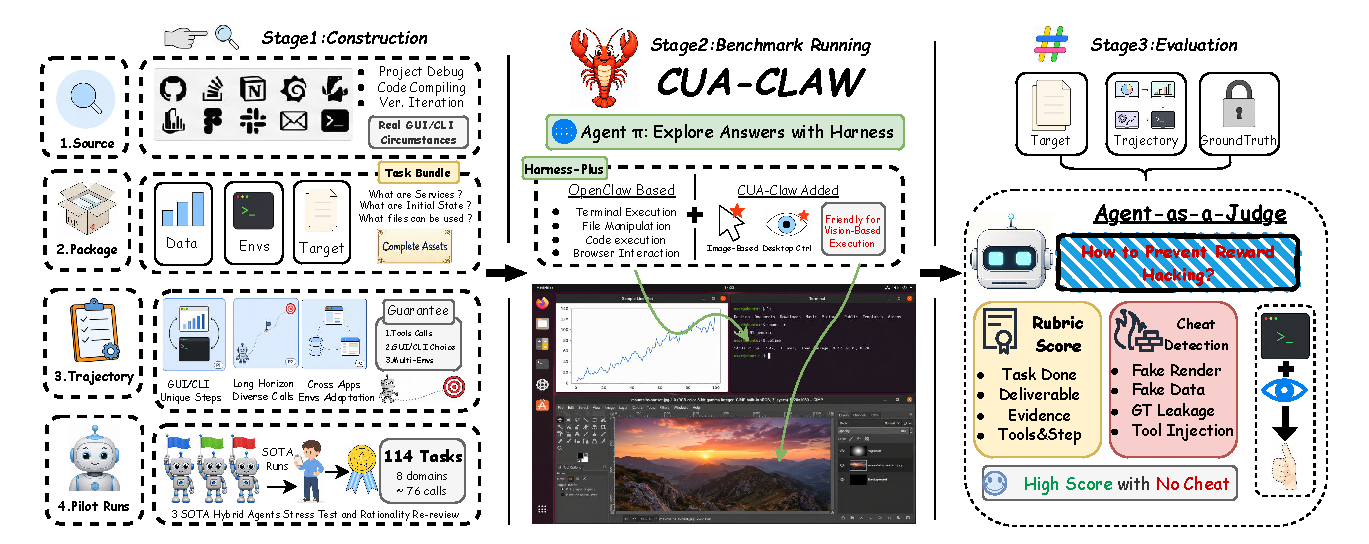
\includegraphics[width=\textwidth]{figures/fig_overview_new.pdf}
\caption{\textbf{\Eyeson{} pipeline.} \textbf{Task:} 114 tasks across 8 domains, harvested from real venues, packaged as $\mathcal{E}=(\mathcal{P},\mathcal{M},\mathcal{C})$ bundles, audited against P1--P3, and stress-tested by $\geq$3 pilot agents. \textbf{Harness:} the agent runs in a single session over an Ubuntu sandbox, where a minimal GUI plugin (one \texttt{screenshot} tool plus nine actuation primitives) is added on top of \textsc{OpenClaw}'s CLI/code tools. \textbf{Evaluation} is performed by an isolated trajectory-aware agentic judge that combines bottom-up rubric scoring with shortcut detection.}
\label{fig:pipeline}
\end{figure*}

\subsection{Task Admission Criteria}
\label{sec:pipeline}

A \textsc{WeaveBench} task is admitted when it satisfies three properties.
\noindent\textbf{P1 Channel non-substitutability:}
Task success must require coordinating GUI observation/action with programmatic modifications through CLI/code operations within the same trajectory.
To make it auditable, each task is annotated with its required single-channel-bound atomic operations (Appendix~\ref{app:p1-falsifier}).
\noindent\textbf{P2 Long-horizon execution:}
The expert reference trajectory must contain multiple interleaved GUI and CLI/code phases rather than a single perception, action, or tool-use step.
\noindent\textbf{P3 Cross-application state:}
The task must span multiple independent applications or processes whose states are linked by the workflow. Agents must preserve and transfer information across these applications, rather than complete the task within a single isolated tool.
Appendix~\ref{app:p2p3-domain} reports trajectory-level evidence for P2 and P3.

\subsection{Task Construction}

Each task is built through a four-stage pipeline.
\noindent\textbf{C1 Archetype-guided sourcing:}
For each domain, experts first define cooperation archetypes that specify the required GUI-side and CLI/code-side roles and then search for real-world tasks from public artifacts (GitHub issues/PRs, postmortems, design mocks, the \textsc{OpenClaw} user community), following the in-the-wild sourcing pattern established by \textsc{SWE-bench}~\citep{jimenez2024swebench}, \textsc{WebArena}~\citep{zhou2024webarena}, and \textsc{OSWorld}~\citep{xie2024osworld}.
\noindent\textbf{C2 Asset packaging:}
For each candidate task, experts assemble a self-contained task bundle. A bundle includes the initial environment, seed data, required assets, user instruction, expected deliverables, expert reference trajectory, and verification anchors used by the judge.
\noindent\textbf{C3 Blind review:} an independent reviewer checks instruction clarity, sandbox reproducibility, P1--P3 validity, and anchor faithfulness.
\noindent\textbf{C4 Pilot validation:}
The three pilot agents are run to detect broken, ambiguous, trivial, or uninformative tasks; pilot outcomes trigger task revision rather than serving as ground truth. The per-venue source breakdown is provided in Appendix~\ref{app:task-sources}.

\begin{figure*}[!t]
\centering
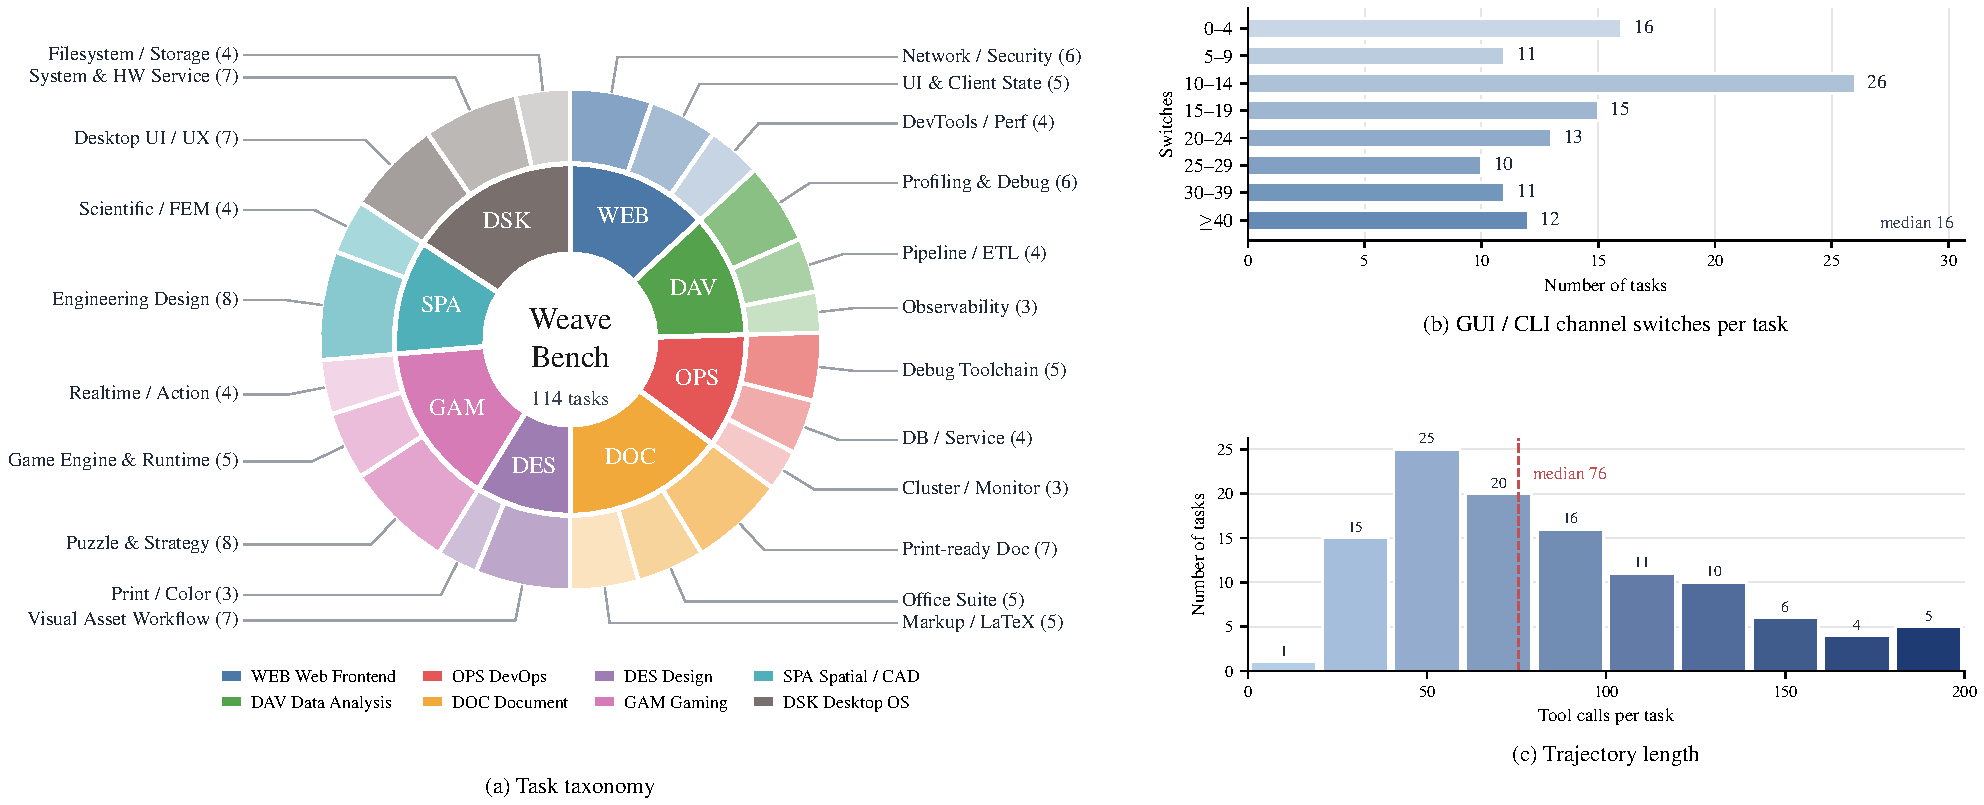
\includegraphics[width=\textwidth]{figures/fig_data_overview_v2.pdf}
\caption{\textsc{WeaveBench} dataset overview. (a) Taxonomy of 114 tasks across 8 domains and 23 subcategories. (b) Number of GUI $\leftrightarrow$ CLI channel switches per task, showing the degree of channel interleaving. (c) Rollout length measured by tool calls in the trajectory.}
\label{fig:taxonomy}
\end{figure*}

\subsection{Task Diversity}
\label{sec:diversity}

\noindent\textbf{Task domains:} \Eyeson{} comprises 114 tasks across 8 real-world work domains (Figure~\ref{fig:taxonomy}(a); Table~\ref{tab:domains}; Appendix~\ref{app:domains}): desktop productivity, document processing, games \& interactive applications, web development, data analysis \& visualization, DevOps \& sysadmin, spatial / 3D / CAD, and design \& creative. Per-domain task counts range from $10$ to $18$, with each domain contributing a distinct cooperation archetype.

\noindent\textbf{Task resources:} Each task is built on real-world assets (code repos, issue threads, monitoring snapshots, design mocks, database dumps, configs) sourced from public venues or replayed in self-hosted sandboxes. Each carries provenance (URL, commit hash, or post id).
The per-venue source breakdown is reported in Appendix~\ref{app:task-sources}.

\noindent\textbf{Trajectory profile:} Tasks are also long-horizon and channel-interleaved: the best live rollouts use a median of $76$ tool calls (max $471$) and a median of $16$ GUI$\leftrightarrow$CLI channel switches per task (Figure~\ref{fig:taxonomy}(b,c); Appendix~\ref{app:p2p3-domain}).

\subsection{Trajectory-aware Agent as Judge}
\label{sec:grader}

Hybrid rollouts cannot be reliably graded from final deliverables alone. In \textsc{WeaveBench}, task success depends on desktop state, source files, generated artifacts, screenshots, and the sequence of tool actions. Final-only grading is therefore vulnerable to shortcuts: artifacts can be synthesized, metrics can be hard-coded, and visually correct states can be reached through specification-violating tool use---instances of the broader \emph{reward hacking} and \emph{specification gaming} failure modes long studied in AI safety~\citep{amodei2016concrete,krakovna2020specgaming}. We therefore treat evaluation as a trajectory-level evidence audit. Each rollout is assessed by a \textbf{trajectory-aware agentic judge} in the spirit of \textsc{Agent-as-a-Judge}~\citep{zhuge2024agentasjudge}, extending the classic \textsc{LLM-as-a-Judge}~\citep{zheng2023llmjudge} and rubric-based G-Eval-style scoring~\citep{liu2023geval} with active evidence re-fetching from artifacts, screenshots, logs, and reference anchors. The task anchors and scoring rules are human-reviewed, and sampled judge verdicts are manually audited.

The judge runs in a fresh subprocess for each rollout, using a fixed backbone and inspection tools for files, images, and shell-based checks. It verifies each case over multiple evidence-gathering turns rather than from a single transcript pass. Runtime details are provided in Appendix~\ref{app:arch}.

Scoring follows a layered pipeline. The judge decomposes each required deliverable into atomic clauses that preserve the instruction's constraints, such as required counts, visual states, file formats, and highlighted regions. It then verifies each clause as satisfied, partially satisfied, or false, citing concrete evidence such as an artifact line, a measured value, a screenshot observation, or a trajectory quote. Clause-level decisions are aggregated into a per-deliverable correctness score $d^{\mathrm{deliv}}_{t,m}$. The judge also assigns eight evaluation dimensions $\{d^{\mathrm{process}}_{t,m,i}\}_{i=1}^{8}$ covering task completion, deliverable correctness, deliverable quality, evidence authenticity, tool-use correctness, final-state correctness, efficiency and robustness, and instruction following. This exposes partial progress while requiring every score to be grounded in inspected evidence. The full rubric is described in Appendix~\ref{app:axes}.

In parallel, the judge scans the trajectory for nine manually confirmed shortcut patterns, including fake screenshots or renders, regenerated fixtures, hard-coded metrics, mock services, duplicate crops, overlay manipulation, ground-truth leakage, and runtime injection---a fine-grained catalog refined from the broader \emph{reward hacking} and \emph{specification gaming} taxonomies of~\citet{amodei2016concrete,krakovna2020specgaming}. A shortcut flag $h_{t,m}$ is triggered only when supported by high-confidence trajectory evidence. If triggered, the rollout receives zero credit. All agents also receive an anti-fabrication policy that prohibits these behaviors while allowing honest skipped-deliverable fallbacks. Details are provided in Appendix~\ref{app:cheats}.

The final score for model $m$ on task $t$ is
\begin{equation}
s_{t,m} =
\begin{cases}
0, & \text{if } h_{t,m}=1,\\
\min\!\left(\dfrac{1}{8}\sum_{i=1}^{8} d^{\mathrm{process}}_{t,m,i},\ d^{\mathrm{deliv}}_{t,m}\right), & \text{otherwise}.
\end{cases}
\label{eq:weave-score}
\end{equation}
The minimum rule prevents strong auxiliary dimensions from masking weak deliverables, while the zeroing rule prevents fabricated or protocol-violating evidence from receiving partial credit.

At the benchmark level, we report two complementary metrics. \textsc{PassRate} measures end-to-end success at threshold $\tau=0.8$, while \textsc{Overall} reports mean partial credit:
\begin{equation}
\begin{aligned}
\mathrm{PassRate}(m)&=\frac{1}{|T|}\sum_{t\in T}\mathbf{1}[s_{t,m}\geq \tau], \\
\mathrm{Overall}(m)&=\frac{1}{|T|}\sum_{t\in T}s_{t,m}.
\end{aligned}
\end{equation}
